% Sets page margins to 1", which is the academic standard
% allows the included extensions of graphic files
% sets graphic path, does not currently work because of space in folder name
% I do not remember what this does
% allows the xhead parameters (text on the top right/left areas of pages)
% \setcounter{tocdepth}{the number of depth}
% INCLUDEGRAPHICS EXPLANATION
% \includegraphics[scale=1]{name of file}
% sometimes you want to twice encase the filename in squiggly brackets. I do not know why but sometimes it is required.


\documentclass{article}
%%%%%%%%%%%%%%%%%%%%%%%%%%%%%%%%%%%%%%%%%%%%%%%%%%%%%%%%%%%%%%%%%%%%%%%%%%%%%%%%%%%%%%%%%%%%%%%%%%%%%%%%%%%%%%%%%%%%%%%%%%%%%%%%%%%%%%%%%%%%%%%%%%%%%%%%%%%%%%%%%%%%%%%%%%%%%%%%%%%%%%%%%%%%%%%%%%%%%%%%%%%%%%%%%%%%%%%%%%%%%%%%%%%%%%%%%%%%%%%%%%%%%%%%%%%%
\usepackage{geometry}
\usepackage{fancyhdr}
\usepackage[pdftex]{graphicx}

%TCIDATA{OutputFilter=LATEX.DLL}
%TCIDATA{Version=5.50.0.2953}
%TCIDATA{<META NAME="SaveForMode" CONTENT="1">}
%TCIDATA{BibliographyScheme=Manual}
%TCIDATA{Created=Monday, January 30, 2012 17:20:46}
%TCIDATA{LastRevised=Tuesday, March 13, 2012 14:14:50}
%TCIDATA{<META NAME="GraphicsSave" CONTENT="32">}
%TCIDATA{<META NAME="DocumentShell" CONTENT="Standard LaTeX\Blank - Standard LaTeX Article">}
%TCIDATA{CSTFile=40 LaTeX article.cst}

\newtheorem{theorem}{Theorem}
\newtheorem{acknowledgement}[theorem]{Acknowledgement}
\newtheorem{algorithm}[theorem]{Algorithm}
\newtheorem{axiom}[theorem]{Axiom}
\newtheorem{case}[theorem]{Case}
\newtheorem{claim}[theorem]{Claim}
\newtheorem{conclusion}[theorem]{Conclusion}
\newtheorem{condition}[theorem]{Condition}
\newtheorem{conjecture}[theorem]{Conjecture}
\newtheorem{corollary}[theorem]{Corollary}
\newtheorem{criterion}[theorem]{Criterion}
\newtheorem{definition}[theorem]{Definition}
\newtheorem{example}[theorem]{Example}
\newtheorem{exercise}[theorem]{Exercise}
\newtheorem{lemma}[theorem]{Lemma}
\newtheorem{notation}[theorem]{Notation}
\newtheorem{problem}[theorem]{Problem}
\newtheorem{proposition}[theorem]{Proposition}
\newtheorem{remark}[theorem]{Remark}
\newtheorem{solution}[theorem]{Solution}
\newtheorem{summary}[theorem]{Summary}
\newenvironment{proof}[1][Proof]{\noindent\textbf{#1.} }{\ \rule{0.5em}{0.5em}}
\geometry{left=1in,right=1in,top=1in,bottom=1in} 
\DeclareGraphicsExtensions{.pdf,.png,.jpg}
\graphicspath{{D:/Dropbox/Private/FP/Gruppe34/FellesDoc/SU_FE3/UseCase/}}
\setlength{\headheight}{15.2pt}
\pagestyle{fancy}
\lhead{Gruppe 34}
\rhead{FP: wat}
\input{tcilatex}
\setcounter{secnumdepth}{1}

\begin{document}


\part{Use Cases}

\section{Creating an Appointment}

\subsection{Use Case Diagram}

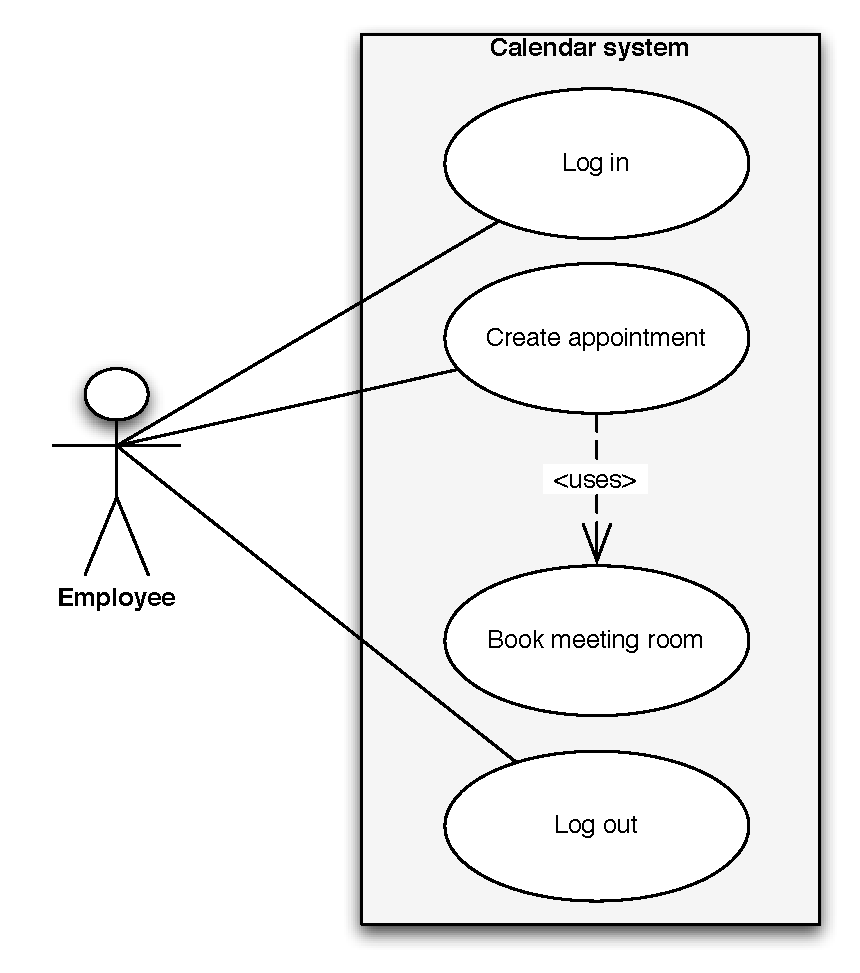
\includegraphics[scale=0.9]{usecaseFP1.pdf}

\section{Calling a Meeting}

\subsection{Textual Description}

\begin{itemize}
\item Create a new meeting.

\begin{itemize} \item Specify date and time.

\item Specify participants.

\item Book meeting room.

\item \textit{Meeting invites are automatically distributed to the
appropriate people.}
\end{itemize}

\item Await response from invitees.

\item React appropriately.

\item \textbf{Receive meeting invitation immediately or upon next use of
system.}
\end{itemize}

\subsection{Use Case Diagram}

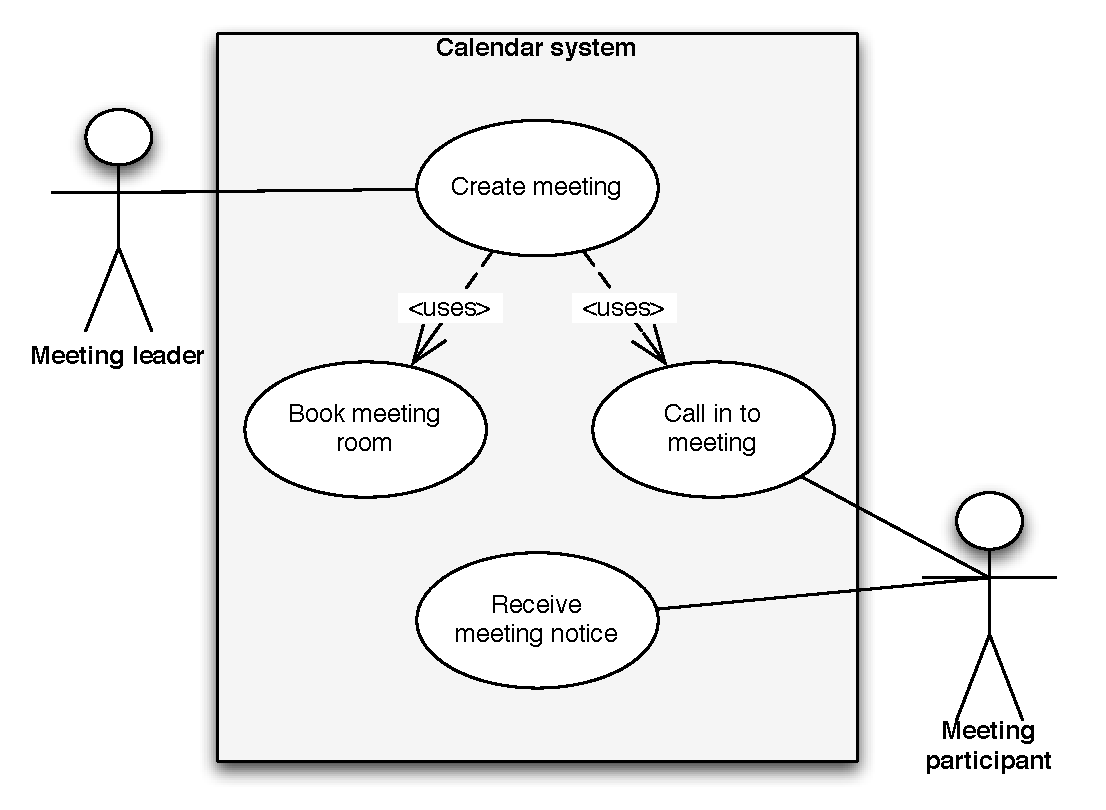
\includegraphics[scale=0.9]{usecase2FP.pdf}

\section{Reacting to Meeting Invite Responses}

\subsection{Textual Description}

\begin{itemize}
\item Receive notification from system that an invitee has rejected the
meeting invitation.
\begin{itemize}
\item Change the meeting's time.

\item \textit{Notifications regarding change in meeting time are
automatically distributed.}
\end{itemize}

\item Await response from invitees.

\item \textbf{Receive notification about an alteration to a meeting's time.}

\item \textbf{Respond appropriately by accepting, rejecting or doing nothing.}

\item Receive response.

\item Remove all invitees that have rejected the invite.
\end{itemize}

\subsection{Use Case Diagram}

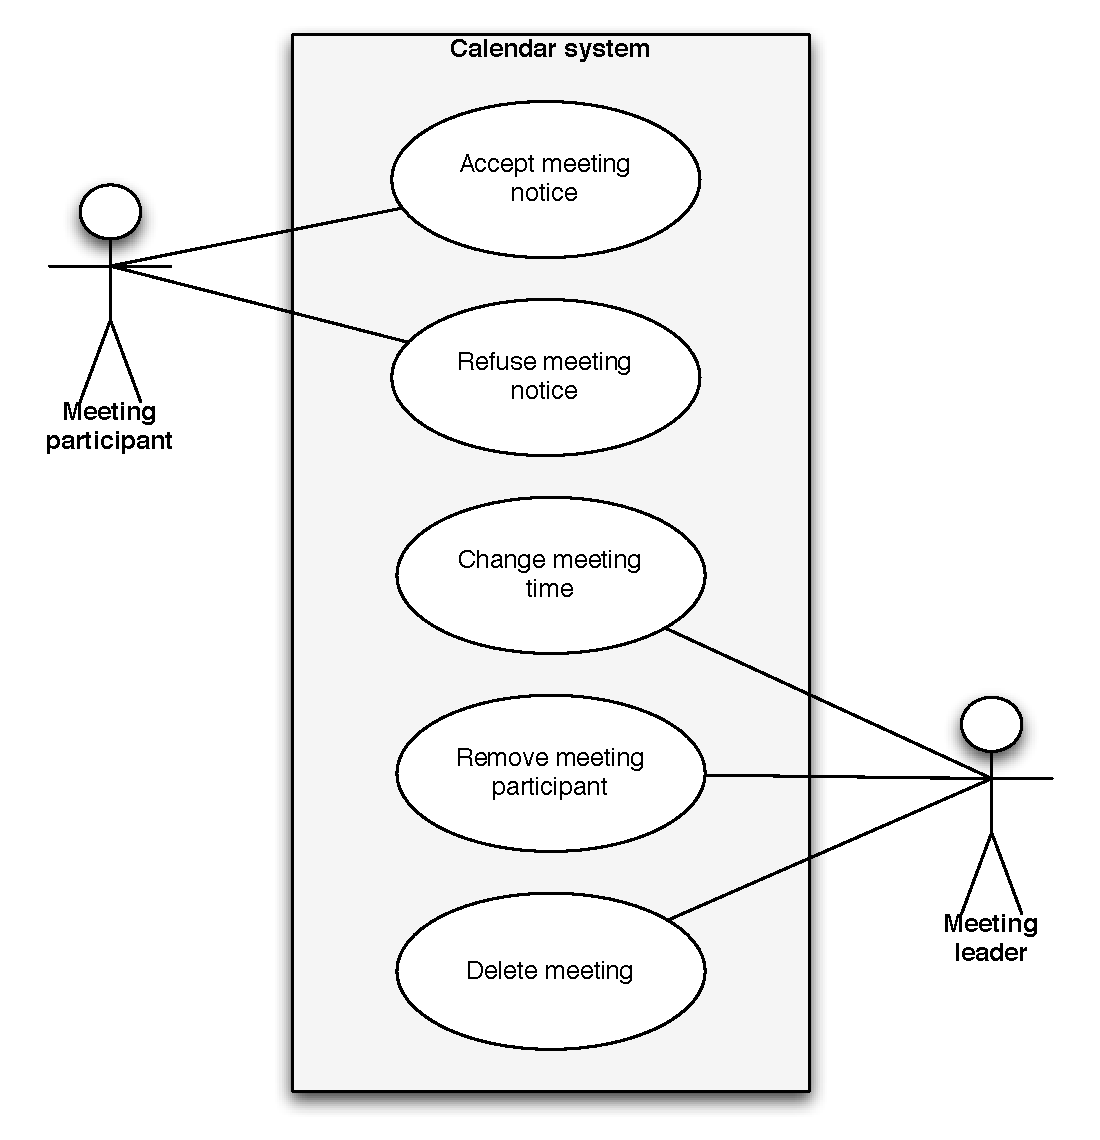
\includegraphics[scale=0.9]{usecase3FP.pdf}

\section{Cancelling a Meeting}

\subsection{Textual Description}

\begin{itemize}
\item Become unable to attend meeting.

\item Cancel meeting by removing it from the calendar.

\item \textbf{Receive notification regarding cancellation of meeting
immediately or upon next use of system.}

\item \textbf{React appropriately.}
\end{itemize}

\end{document}
